\section{Faithful to Love}

\begin{quotex}
The various ladies celebrated by the poets attached to the mysterious organization of the Fedeli d'Amore, from Dante, Guido Cavalcanti, and their contemporaries, to Boccaccio and Petrarch, are not women who actually lived on this earth but are all under different names, one and the same symbolic Lady who represents transcendent Intelligence or Divine Wisdom. \flright{\textsc{Rene Guenon}, \emph{The Secret Language of Dante}}

\emph{O voi che avete gl'intelletti sani, Mirate la dottrina che s'asconde Sotto il velame delli versi strani !}

O you who have healthy intellects, look at the doctrine that lies hidden under the veil of mysterious verses. \flright{\textit{Inferno IX}}

Women's strength lies in her beauty, whereas Man's beauty lies in his strength. \flright{\textsc{Boris Mouravieff}}

He who knows himself knows God. \flright{\textsc{Clement of Alexandria}}

\end{quotex}
\paragraph{Esoteric Schools}
Guenon's written works are often dry and intellectual, which have opened him up to the charge of “rationalism”, so it may be easy to miss his point regarding the Fedeli d'Amore. Yet that is where we need to look in order to understand initiation in the West. He goes further, and adds the stories of Chivalry, the search for the Grail. Even \emph{The Romance of the Rose}, translated into Italian by Dante, is a work that hides its hidden doctrine. Historians dismiss it as a work of popular entertainment. Who has bothered to read it; and of those who have read it, who has understood it?

The Persian poets, like Rumi and Hafiz, need to be penetrated to reveal the secret doctrine. Such poets influenced the Sicilian poets from whom Dante was initiated. Hafiz was the equivalent of today's pizza delivery guy. Yet, like the Buddha who sat under the fig tree until he was enlightened, Hafiz did a vigil for 40 nights at the tomb of a Saint with the same effect.

Guenon asserts that from Pythagoras to Virgil to Dante, the chain of Tradition was never lost on Italian Soil. This Tradition was continued by the alchemists with their quest for the Mystical Marriage. More recently Vladimir Solovyov brought us revelations of Divine Wisdom. Carl Jung, in a scientific way, has recovered the hidden doctrine of the alchemists, even recreating the pathway to the Mysterium Coniunctionis.

As a student of science, I learned to keep a lab book of experimental results. The science of alchemy is no different. It may be helpful to share the results of alchemical experiments in a concrete way rather than in abstract, intellectual terms. Our age is more open and I have learned that some things remain hidden out in the open. There are those who just don't see it. This will involve “women who actually lived on this earth” and some who have not, at least not as I have experienced them.

\paragraph{Basic Instinct}
\begin{quotex}
The more civilized, the more unconscious and complicated a man is, the less he is able to follow his instincts. His complicated living conditions and the influence of his environment are so strong that they drown the quiet voice of nature. Opinions, beliefs, theories, and collective tendencies appear in its stead and back up all the aberrations of the conscious mind. \flright{\textsc{Carl Jung}, \emph{Aion}}

\end{quotex}
Sometimes you need to live your life in reverse. What was it like before opinions, beliefs, and theories filled your mind? What were your first instincts as a boy? I grew up with my Nana, Mother, and Sister; they mostly stayed at home, while I, along with the other boys, would be gone for hours. We would play games, wander, fight, explore. But I could always count on a home to return to. I envisioned myself as a caveman. I would go out, confident that I could return to a warm cave. Nana would make me what my father called “peasant food”; tasty and comforting but not available in restaurants. That includes gnocchi which she made by hand. Now gnocchi are the rage, overpriced and mispronounced as “noki”.

Nana, Mother, and Sister had special roles in my life. All the other girls were fair game, mostly indistinguishable from each other. Their thoughts were mysterious, even alien, but of little interest. In Kindergarten, we had dance time in which the girls rushed to pick a partner. Two of them ran to me. A shoving match ensued and one was pushed to the ground. I didn't understand the fuss since I didn't even like to dance.

That world for me, was impervious to intellectual abstractions. It was populated by angels, demons, saints, Jesus, Mary, God, suffering and triumphant souls, prayers, holy days, fasts, abstinence, and so on. Mary has watched over me my whole life or else I'd be dead by now.

\paragraph{Remote Control}
I can wave my hand, shake a leg, and nod my head. Yet there is one appendage over which I have no conscious control. There was a point when I came to realize that another being, through her touch, or even seeing or imagining her, could make it rise and fall, like the way the Moon controls the tides. Except that the Moon is always there, but a woman needs to be pursued.

That led to years of wandering outside the cave. I had to learn many new skills in order to survive. I learned how to dress, learned to dance, worked out, took acting lessons. Through spiritual practices, I developed more control over thoughts and emotions. In particular, I had more options to express a Persona before reverting to my rather Saturnine default personality.

There were too many risks, things I did that I would not have done even to save my own life. If you've ever had to crawl out a bedroom window or scamper down a fire escape in the middle or the night, you will understand. Like encountering a rusalka, pleasure and risk interpenetrate each other.

\paragraph{Penetration}
At a certain point, it just becomes tedium, without a purpose. Then mere penetration is not enough with someone you love – or think you love. Your desire then is to penetrate her soul; that is what is needed, even if the reasons are unclear. Skin, which a moment ago was an organ of intense pleasure, suddenly becomes an obstacle. The frustrating conclusion is that the soul is impervious to physical contact.

At the level of the psyche, the roles are reversed: the woman becomes the active principle and the man passive. This is known in Tantra; \textbf{Francesco da Barberino}, also in initiate into the Fedeli d'Amore, reveals it in \emph{Documenti d'Amore}:

\begin{quotex}
the man with his passive intellect is reunited with the active intelligence, represented by woman 

\end{quotex}
Tomberg expresses it like this:

\begin{quotex}
the intellect is the feminine side of the soul, whilst the fertilising imagination is the masculine principle 

\end{quotex}
Expressed another way, the Anima is the passive receptor of images revealed to him by the woman. Once again, another being is in control, in this case, of the most intimate parts of a man's soul.

\paragraph{Imagination and Inspiration}
\begin{quotex}
The intellect that is not fertilised by imagination guided by the heart is sterile. It depends on impulses which it receives from the participation of the heart by means of the imagination. \flright{\emph{Meditations on the Tarot}}

\end{quotex}
The scholastic principle is that knowledge begins in the senses; from that base one may be led to the knowledge of the ideas. Some few will go beyond even that to an intuition, a direct knowing, of what is beyond even the ideas.

Analogously, spiritual ideas are first expressed in images, symbols, legends, and the like. These excite the Imagination, which is sufficient to most people. Some few will persist in understanding those figures in the imagination.
\begin{wrapfigure}{rt}{.3\textwidth}
 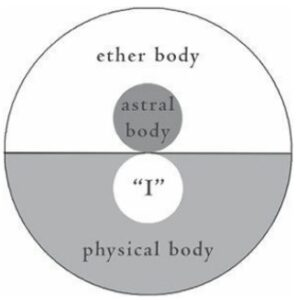
\includegraphics[scale=.5]{a20201211FaithfultoLove-img001.jpg}
\end{wrapfigure}
That leads to the stage of Inspiration. To return to the original idea, Dante started with the image of Beatrice who was not a real woman, or at least not real to him. Nevertheless, that inspired a huge creative output of philosophy and poetry, culminating in his masterpiece.

The final stage is Intuition, when he reaches into the highest heavens. In Intuition, the whole is grasped all-at-one, in its entirety. That is a long way from the physical effects that Beatrice's beauty elicited from him in his youth.

\paragraph{Individuation}

The process of Individuation involves the four primary archetypes: Ego, Shadow, Anima (or Animus), and Self. The intent is not to psychologize the attainments of the initiates. Nevertheless, the journey of the Spirit will have its reflection in the Soul. Therefore, it is helpful to focus on phenomenological experiences, even if, ultimately, they are left behind. That occurs when Inspiration becomes Intuition, that is, the help of sensory images or thoughts are no longer necessary.

The path can be summarized, referring to the diagram on the right (from Valentin Tomberg):

\begin{itemize}
\item \textbf{Ego}: The I of the body, attentive to its needs. What is above the line is unconscious to it. 
\item \textbf{Shadow}: The knowledge of good and evil requires an adversary to push back. Catherine of Emmerich reveals this as an evil being, but not irredeemably evil. 
\item \textbf{Anima}: The unity is broken. A person of the opposite sex reunites. 
\item \textbf{Self}: The return to the Primordial State requires these elements to be integrated in the Self, represented by the circle. 
\end{itemize}
\paragraph{Ego}
As Jung defines it, the Ego

\begin{quotex}
forms the centre of the field of consciousness; and, in so far as this comprises the empirical personality, the ego is the subject of all personal acts of consciousness. 

\end{quotex}
The Ego can arise only through thinking. Descartes' insight — \emph{I think, therefore I am} — is correct. The intellectual soul is tied to the Ego. That is the spirit breathed into man that lights up consciousness; actually, the source of the light is the Holy Spirit. As the diagram shows, the undeveloped Ego is the I of the body. The etheric and astral bodes (vegetative and animal souls) are unconscious to it.

The esoteric student will be encouraged to recall the first time he had the awareness of being an I, i.e., a separate being. The long-term task is to bring the unconscious into awareness. This will develop a stable Self and beyond that, even higher states of being.

\paragraph{Shadow}
\begin{quotex}
The shadow is a moral problem that challenges the whole ego-personality, for no one can become conscious of the shadow without considerable moral effort. To become conscious of it involves recognizing the dark aspects of the personality as present and real. \flright{\emph{Aion}}

\end{quotex}
Young children act spontaneously; there is no separation between emotion and response. Traditionally, there is no moral responsibility until around the age of seven. Thus, in the exoteric tradition, children begin confession at that age; that trains them in the task of becoming conscious of the Shadow.

Yet even that is insufficient. All negative emotions and thoughts, idle fantasies, and the like need to be brought into awareness.

\paragraph{Anima}
This is actually the Syzygy Anima-Animus, but I can only write from the male perspective. The Anima is the most difficult archetype to recognize. Like the physical member that requires a partner to be aroused, so also does the Anima. Mother, Nana, and Sister are the first to contribute to it.

\begin{quotex}
The mother carefully inculcated into him the virtues of faithfulness, devotion, loyalty, so as to protect him from the moral disruption which is the risk of every life adventure. \flright{\emph{Aion}}

\end{quotex}
Nevertheless, to remain at that level is be infantile, so there must be more. The Anima contains the imagoes of Baubo, all his lovers, Divine Wisdom. Baubo returns in the infamous interrogation scene from \emph{Basic Instinct}. She is hardly safe and consistent.

\begin{quotex}
This perilous image of Woman belongs to him; she stands for the loyalty which in the interests of life he must sometimes forgo; she is the much needed compensation for the risks, struggles, sacrifices that all end in disappointment; she is the solace for all the bitterness of life.

And, at the same time, she is the great illusionist, the seductress, who draws him into life with her Maya — and not only into life's reasonable and useful aspects, but into its frightful paradoxes and ambivalences where good and evil, success and ruin, hope and despair, counterbalance one another. Because she is his greatest danger, she demands from a man his greatest, and if he has it in him, she will receive it. \flright{\emph{Aion}}

\end{quotex}
Recall my childhood vision of the cave; the boy could wander about in the world and take risks, certain that he could find comfort and solace on his return. Now that the primal cave no longer exists, that boy needs to build his own cave and find a new source of solace.

Ancient myths, legends, and tales of chivalry portray tales of men having to prove themselves to his potential lover through various tasks, such as feats of bravery, strength, speed. Or perhaps he will praise her beauty and immortalize her in poems and stories. But she needs to be worth the trouble and few are.

The psychological process becomes complicated since it involves a quaternity: the real man and woman, the Anima, and the archetype of the Wise Old Man (or the Animus and archetype of the Chthonic Mother, often represented by Hecate).

That is why, esoterically, the actually existing woman can be a hindrance. The merely psychological level must be transcended. Then higher forces come into play: the Holy Spirit and Divine Sophia or Wisdom. Nay, they are not archetypes, but rather spiritual realities. Psychologically, the Anima is perturbed with “frightful paradoxes and ambivalences”, and other psychic oscillations. The Holy Spirit is the light of consciousness, Wisdom is His reflection in the Anima. When the waters of the Anima are unperturbed, it perfectly reflects the Holy Spirit and something higher can be born.

\paragraph{Self}
Before the Shadow and Anima are integrated into consciousness, the true Self is also unconscious. The Ego believes he is “in charge”, even while he is buffeted by forces that are unknown or unclear to him. As the diagram above shows, the I needs to become master of the unconscious elements of the etheric and astral bodies. Unfortunately, this final stage of integration has its own dangers, so help is often required along the way.

\begin{quotex}
It is of the greatest importance that the ego should be anchored in the world of consciousness and that consciousness should be reinforced by a very precise adaptation. For this, certain virtues like attention, conscientiousness, patience, etc., are of great value on the moral side, just as accurate observation of the symptomatology of the unconscious and objective self-criticism are valuable on the intellectual side. \flright{\emph{Aion}}

\end{quotex}
This psychological Self is still short of the final goal. By transcending the psychological level, higher levels of the Self, with more integration, can be achieved. Ultimately, it leads to life before the Fall, the return to the Primordial State:

\textsc{Et incarnatus est de Spiritu Sancto ex Maria Virgine}.

\begin{quotex}
[The above formula] contains the trinity of the generator above, of the generant below, and the generated—or: the Holy Spirit, the Holy Virgin and the God-Man. It is at the same time the formula of sacred magic in general, because it expresses the mystery of the union of divine will and human will in the element of blood. \flright{\textsc{Valentin Tomberg}, \emph{Meditations on the Tarot}}

\end{quotex}
Esoterically, blood is the physical organ of the human I.

Man is made in the image of God; the Self is the image of Christ in the soul.

\paragraph{Appendix: Polar Beings}
Often the guys will ask how they can get their girlfriends involved in their path. From experience, I don't see how that can be done. If you get along with your gf and she does not oppose your spiritual quest, that is probably a big success.

The esoteric teaching is that many women may be compatible physically but a much smaller number will be a good match for the soul. But there is only one Eve for Adam; she is your polar being. You will meet her once in your life. I suspect most of you have met her already, and are even with her now without fully realizing it. You need to be fully conscious to see it clearly. She may not be a woman “just like you”, or how you think you are; rather, she will be just like your Anima. The more conscious you are of the Anima, the better will you recognize her.

Two souls who fully know each other become, in effect, a single I. This is the highest path.



\flrightit{Posted on 2020-12-11 by Cologero }

\begin{center}* * *\end{center}

\begin{footnotesize}\begin{sffamily}



\texttt{Sibylle on 2020-12-23 at 07:46 said: }

Thank you very much for this article. I do hope it will resonate with many readers. It certainly touched me since from the practical female perspective relationships remain very much stuck due to the lack of response a woman gets from the soul of a man. (And as a result of that even the “remote control” loses its power, which in turn is interpreted as homo-bi-trans-whatever-sexuality whereas it is just a sign of the enormous distance a man put between himself and his body, let alone his soul.)

What if the cave is a cave full of men instead of women because men went into hiding? It seems impossible to find a woman resembling a man's “Anima” if men refuse to leave the cave and allow that space to women. Of course you are talking about a man's perspective and I absolutely understand that men are afraid of women. Especially nowadays with all this obnoxious behaviour by many females.

It really doesn't contribute to a greater depth of a relationship though if men refuse to take care of themselves. The so called risk taking mentioned in this post does not happen anymore. As a result women need to compensate for the lack of respect men show towards themselves which makes any real intimacy impossible, because the active role becomes the woman's role all along, not only when it comes to the level of the psyche. This change of behaviour makes attraction impossible even before the level of the soul is reached. Sexual attraction cannot arise when a woman needs to make up for a man's missing self respect.

We all know the causes for this mess. However – “feminism” could never have happened with the enormous help of many so called intelligent men who could and should have known better. (But as we know: Every vote counts!) It cannot be left to women alone to clean up the mess. We need a hand. There can be no deeper revelation if there is no quest. Rusalka is a necessary first step. It is impossible to submit oneself if there is nothing to submit to. And believe me, the need for submission has never been greater (as mentioned here\footnote{\url{https://www.gornahoor.net/?p=8417}}).

It is something women give with great joy and very freely if there happens to be a receiver. However it is an act that arises from the occasion where it is needed, it can neither be forced nor demanded.

The “right” woman can only be “right” if she is needed. She can only be needed by someone who has left his cave. If you decide to stay in there, she cannot find you.

In this sense remainig faithful to love means remaining faithful to oneself in allowing this self to be known to itself before it can be revealed to others (a woman). When men don't bother about themselves and remain in their caves women become superfluous. It's planet Adam without the need for any sort of Eve. So imagine what it feels like to be a woman on such a planet. Everything a woman does can been accomplished better by a man. Even remaining in the cave. So why do we exist?


\hfill

\texttt{Cologero on 2020-12-23 at 17:27 said: }

The knight Don Manuel de Leon retrieved a glove from a lion's cage at the request of a Lady. He then slapped her for frivolously endangering the live of a knight.


\hfill

\texttt{Sibylle on 2020-12-24 at 08:11 said: }

This slap probably taught the Lady more than a thousand words about the moral implications of her carelessness. Women never understand the effect they have upon men unless they receive their initiating slap. It is rather an act of information than of dominance.

The Lady will surely have remembered that Knight's slap as one of the most caressing moments of her life.


\hfill

\texttt{Santiago on 2022-06-07 at 00:21 said: }

“…she is the solace for all the bitterness of life.

And, at the same time, she is the great illusionist, the seductress, who draws him into life with her Maya…”

Why must the Anima be both `Madonna' and `Whore'. How is it even possible for her to take up such a contradictory existence? In both dreams and real life, women are capable of the most radical transformations. I don't know how it's even possible to be both so enraptured by someone and yet to be made to experience such fear.

“The Anima contains the imagoes of Baubo, all his lovers, Divine Wisdom. Baubo returns in the infamous interrogation scene from Basic Instinct.”

Some lovers moreso than others; some I will never get over. Mainly from the perspective of dreams, the Anima's relationship with time is also worthy of note. Little forgotten details from years ago will be brought up, or I'm given little premonitions related to the upcoming days or weeks. Sometimes the similarities are even undeniable, beyond coincidence. It's like a game to her, and she responds to the interest I take.

And you hit the nail on the head. Every now and then, something analogous to the Basic Instinct scene does occur, but if I take the bait, holy hell does she make me pay for it. FWIW, I'm never allowed beyond that point. It's like a cruel test.

“The psychological process becomes complicated since it involves a quaternity: the real man and woman, the Anima, and the archetype of the Wise Old Man.”

Kind of a technical queston, but who is the `Wise Old Man'. and how is he related to all this?


\hfill


\end{sffamily}\end{footnotesize}
